\documentclass{article}
\usepackage[utf8]{inputenc}
\usepackage{imakeidx}
\makeindex
\usepackage{graphicx}
\graphicspath{ {./images/} }
\usepackage{float}
\usepackage{amsmath}
\usepackage[colorlinks, linkcolor=blue]{hyperref}
\usepackage[italian]{babel}
\usepackage[backend=biber]{biblatex}
\usepackage[autostyle,italian=guillemets]{csquotes}
\addbibresource{sample.bib}
\usepackage{booktabs}
\usepackage[left = 3.8 cm, right = 3.8 cm]{geometry}

\title{\huge Stima della soglia di ablazione}
\author{ \large Onofrio Davide Caputo \\ \large Giuseppe Giorgio  \\ \large Francesco Pio Merafina}
\date{ \small Data esperimento: 6 Maggio 2022 \\ Data relazione: 10 Maggio 2022}

\begin{document}
\begin{figure}[t]
\hspace*{-2cm}
    
\includegraphics{Uniba.png}
\end{figure} 
\maketitle

\noindent \textbf{\Large Abstract}\\

\noindent L'utilizzo dei laser come strumenti per incidere, tagliare o forare materiali passa necessariamente per la rimozione del materiale in eccesso. L'esperienza qui presentata mostra come, affinché si possa ottenere un'ablazione, sia necessario superare una determinata soglia, al di sotto della quale, pur illuminando il materiale, esso non viene danneggiato. 
La stima di questa soglia sarà oggetto della relazione. 

\tableofcontents

\normalsize
\setlength{\columnsep}{20pt}
\twocolumn
\section{Introduzione}
La grandezza di cui si vuole stimare la soglia è detta fluenza e non è altro che il rapporto tra energia incidente su una certa area e l'area stessa. 
Per un fascio gaussiano la fluenza ha un andamento esponenziale; il valore di picco è indicato come $F_0$, mentre si indica con $F_th$ il valore di soglia sopra il quale si ha danneggiamento del materiale e quindi ablazione.
Si noti che nel caso di fluenze di soglia pari alla fluenze di picco, sul materiale risulterà danneggiata una porzione sferica di raggio nullo.
É possibile connettere il diametro del foro ablato sul materiale con il valore della fluenza di soglia mediante la formula \ref{fomula diametro fluenza}.

\begin{equation}
    D^2 = 2w^2 ln (\frac{F_0}{F_{th}})
    \label{fomula diametro fluenza}
\end{equation}

É inoltre possibile esprimere la fluenza di picco $F_0$ in termini dell'energia dell'impulso $E_P$, come mostrato nella formula \ref{fomula fluenza di picco} :

\begin{equation}
    F_0 = \frac{2E_P}{\pi w^2}
    \label{fomula fluenza di picco}
\end{equation}



\section{Descrizione dell'apparato sperimentale}
L'apparato sperimentale consiste di una sorgente laser polarizzata orizzontalmente, che produce un fascio impulsato ad una frequenza di ripetizione $f_{rip} = 200 kHz$ nell'infrarosso, in particolare ad una lunghezza d'onda di $\lambda = 1030 nm$.
Il fascio inviato dalla sorgente viene deviato da uno specchio posto a 45°, entra in un modulo contenente lamine a mezz'onda e un polarizzatore che riportano il fascio orizzontale e che all'occorrenza ne riducono la potenza.
Successivamente c'è un altro specchio a 45° e infine un modulo che alza il fascio verso l'alto, portandolo all'altezza di un traslatore x,y,z, dotato di viti micrometriche, per aggiustare la posizione del campione.

Il controllo del fascio è gestito da un software che permette di decidere la potenza del fascio e la forma della figura che si vuole incidere.

\section{Descrizione dell'esperimento}
L'esperimento consiste in una iniziale presa dati della potenza del fascio laser.
In particolare, in corrispondenza di un valore percentuale scelto, si misurava, mediante un power meter, la potenza del fascio che sarebbe andato ad incidere sul campione. Sono stati misurati 8 valori di potenza.
Successivamente è stata condotta la lavorazione vera e propria, utilizzando i valori di potenza misurati ed effettuando 5 fori per potenza.
Alla fine della lavorazione sono state misurate nuovamente le potenze del fascio.

Ultimata la fase di lavorazione, si è provveduto alla misura dei diametri dei fori mediante un microscopio dotato di software di misura al computer.
I dati ottenuti sono riportati nella sezione seguente.


\section{Analisi dei dati}
Si riportano in tabella \ref{potenza} la due misure di potenza iniziale e finale, il valore medio e l'errore massimo.
\begin{table}[h!]
\centering
\begin{tabular}{llll}
$P_{in}$   & $P_{fin}$  & $\Bar{P}$  & $u_P$  \\
\hline
0.238 & 0.249 & 0.244 & 0.006 \\
\hline
0.320 & 0.330 & 0.325 & 0.005 \\
\hline
0.400 & 0.410 & 0.405 & 0.005 \\
\hline
0.480 & 0.490 & 0.485 & 0.005 \\
\hline
0.560 & 0.570 & 0.565 & 0.005 \\
\hline
0.695 & 0.700 & 0.698 & 0.003 \\
\hline
0.806 & 0.820 & 0.813 & 0.007 \\
\hline
0.966 & 0.982 & 0.974 & 0.008
\end{tabular}
\label{potenza}
\caption{Tabella dei dati delle potenze.}
\end{table}

Dalla formula \ref{fomula diametro fluenza}, si esegue una linearizzazione nel modo seguente:



\begin{equation}
\begin{split}
    D^2=2\omega^2 log(\frac{F_0}{F_{th}})= \\ 2 \omega^2 (log(E_P)-log(\frac{\pi \omega^2 F_{th}}{2}))= \\
    Alog(E_P) - Alog(\frac{\pi A F_{th}}{4}) \equiv Ax+B
\end{split}
\end{equation}

Dove $A=2\omega^2$ e $B=-Alog(\frac{\pi A F_{th}}{4})$.
\\

Il quadrato dei diametri dei fori ottenuti è stato rappresentato in funzione del logaritmo di $E_P$, a sua volta ricavato come rapporto di $P_{med}$ e $f_{rip}$.
I dati sono stati interpolati da una retta $y = Ax + B$ e i parametri A e B sono stati usati per ricavare la fluenza di soglia.

\begin{figure}[h!]
    \centering
    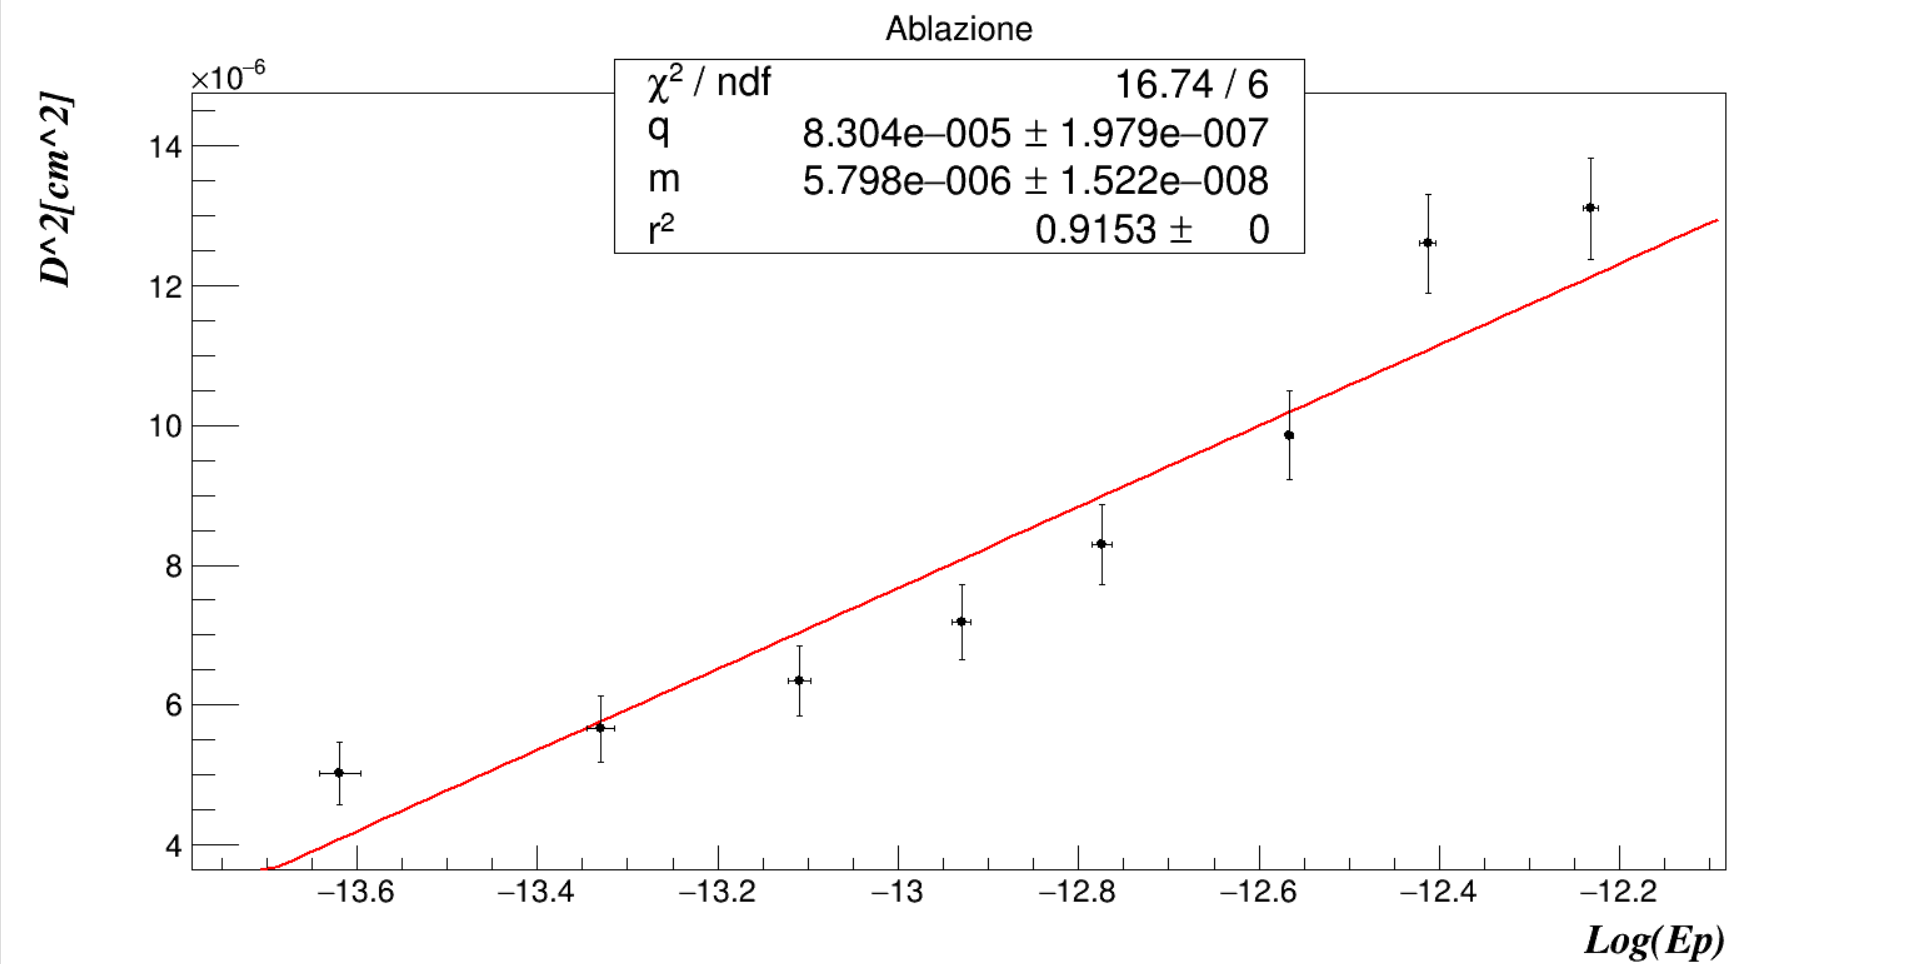
\includegraphics[width=1.1\linewidth]{Ablazione.png}
    \caption{Grafico ablazione. Nella legenda i parametre m e q sono i corrispondenti di B e A}
    \label{figura_ablazione}
\end{figure}


\section{Conclusioni}

Dalla definizione di B si ottiene che:
\begin{equation}
    F_{th}=\frac{4}{\pi A} exp(-\frac{A}{B})
\end{equation}
Dai dati ottenuti, il valore della soglia di ablazione ottenuto corrisponde a:
\begin{equation}
    F_{th}=9.12 \cdot 10^{-3}\pm 1.1 \cdot 10^{-7} J/cm^{2}.
\end{equation}







\end{document}
